\section{Das Ausweichlager Rennersdorf}

Die Überlebenden des Todesmarsches kamen am 23. Februar in das unweit von Herrnhut\index{o}{Herrnhut} gelegene Rennersdorf. Die SS quartierte die Häftling in einem alten herrschaftlichen Gutshof am Fuße des Berges Eichler ein.
Das sogenannte Gut Oberrennersdorf (Bild ~\mypicsref{gutoberrennersdorf}) befand sich seit 1765 im Besitz der Brüder-Unität Herrnhut\index{o}{Herrnhut}.
Unter dem Vorwand der Knappheit von Siedlungsland und der strategischen Lage in Grenz\-nähe zur Tschechoslowakischen Republik erwirkte die Wehrmacht nach zähen Verhandlungen den Verkauf des Gutes Oberrennersdorf als Bestandteil des Remonteamtes (zusammen mit dem Berthelsdorfer\index{o}{Berthelsdorf} und Großhennersdorfer Gut) am 3. März des Jahres 1937\footnote{UArch 7275.}. Dem damaligen Pächter Rosenberg wurde im Juli des selben Jahres gekündigt\footnote{Ebenda}. 
Das tote wie auch das benötigte lebende Inventar ging in den Besitz der Wehrmacht über. Die landwirtschaftlichen und forstwirtschaftlichen Unternehmungen setzte man fort, wobei die Pferdeaufzucht eine wesentliche Rolle spielte. 
Laut dem Rennerdorfer Ortschronisten war der damalige Wirtschaftsvogt und Betriebsführer ein gewisser Reinhold Lehmann\index{p}{Lehmann, Reinhold}\footnote{Vgl. Robert Heinze: Ortschronik Rennersdorf. Reinhold Lehmann (*26.03.1889) war eines von insgesamt 60 NSDAP Mitgliedern im Ort, die im Zuge der Entnazifizierung durch die sowjetische Militärkommandantur ermittelt wurden. KArchLZ Rennersdorf / 142. }. Außer ihm wohnten noch eine Reihe anderer Personen auf dem Gut: der Tierarzt Zwerschke mit seinem Sohn, ein Schäfer namens Schlaffke sowie die Familien Bittrich, Feder, Engel und Weber. 

\paragraph{Welcher Art war das Lager in Rennersdorf?} Genau wie das hier bereits behandelte Görlitzer Lager im Biesnitzer Grund, ist das Lager in Rennersdorf definitionsgemäß kein Konzentrationslager\footnote{Im Sinne der Inspektion der Konzentrationslager von Oswald Pohl.}. Ebenso wenig kann man es als Arbeitskommando bezeichnen, da nur geringfügige Arbeitseinsätze erfolgten. 
Vielfach wurde das Lager in der Literatur als KZ-Außenlager bezeichnet, wobei es jedoch, entgegen Isabell Sprengers Annahme, kein reines Männerlager war\footnote{Vgl. Isabell Sprenger: Groß-Rosen, S. 232.}. Angesichts der Tatsache, dass die Gefangenen nur für knapp zwei Wochen in Rennersdorf verweilten und anschließend wieder an ihren Ausgangspunkt nach Görlitz zurückkehrten, scheint es im wörtlichen Sinne ein Ausweichlager gewesen zu sein. Im Archiv des KZ Groß-Rosen\index{o}{Groß-Rosen} sowie in den Verwaltungsbüchern der Gemeinde Rennersdorf existiert kein einziges Dokument, was den Zusammenhang mit dem Hauptlager erkennen lässt. Belegt ist hingegen der enge Kontakt zwischen den Kommandoführern der Evakuierungsmärsche und dem Meldekopf des Stammlagers, welcher sich ab dem 17. Februar 1945 im Außenlager Reichenau im Sudetengau (Rychnov u Jablonce nad Nisou, Tschechien)\index{o}{Reichenau} befand. 
Im Folgenden wird das Lager in Rennersdorf dennoch als KZ-Außenlager bezeichnet, um damit einerseits den Charakter eines KZ-Lagers auszudrücken und andererseits eine von der Existenzdauer unabhängige Benennung beizubehalten\footnote{Gleiches gilt für das KZ-Außenlager Kunnerwitz, wo bereits vor dem Durchmarsch der Görlitzer KZ-Häftlinge ein Groß-Rosener Arbeitskommando bestand. Sohland am Rotstein, als zweite Station während des Todesmarsches von Görlitz nach Rennersdorf, soll jedoch nicht als KZ-Außenlager angesehen werden, da die Gefangenen dort nur einen Tag verweilten und kein geordneter Lagerbetrieb errichtet bestand.}. 
%Offenbar gab es für diese einzige Einquartierung von KZ-Häftlingen eine Übereinkunft zwischen SS oder der Görlitzer Kreisleitung und der Wehrmacht als Eigentümer der Gebäude und Ländereien. 


\begin{figure}[htb]
    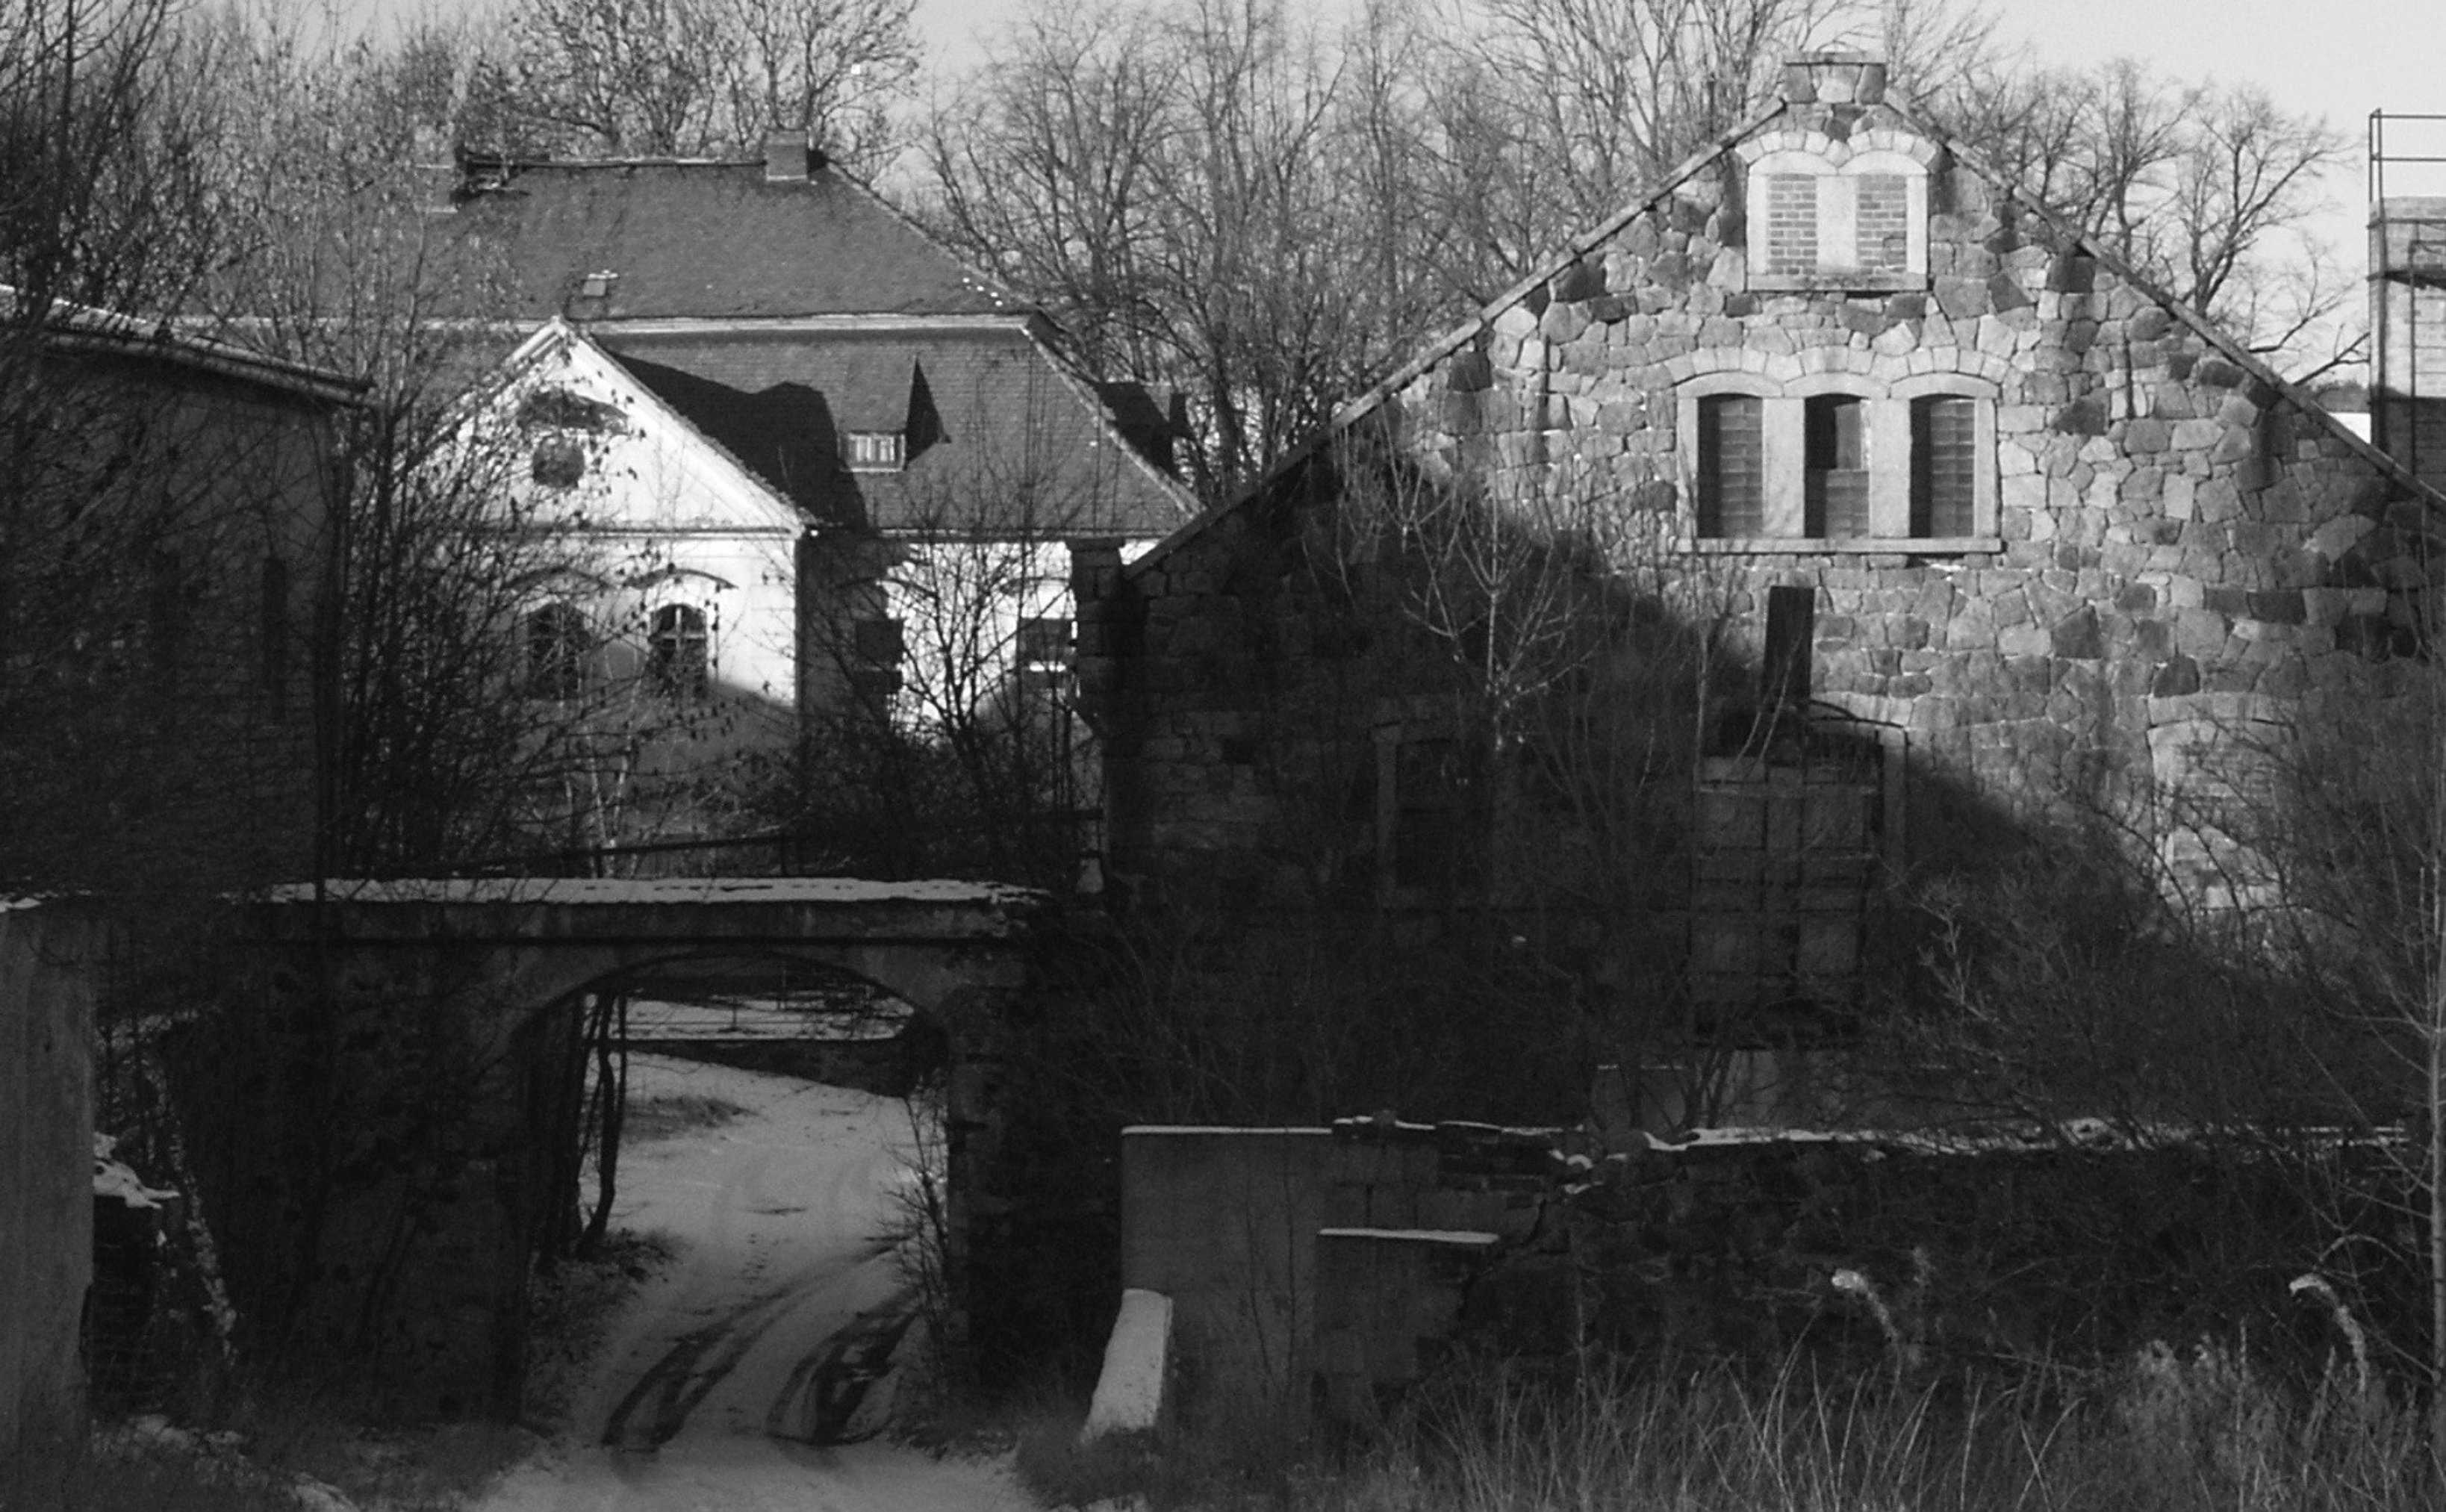
\includegraphics[width=\linewidth]{images/renn01}
    \caption[Gut Oberennersdorf]{Das Gut Oberrennersdorf}
    \label{gutoberrennersdorf}
\end{figure}



%%%%%%%%%%%%%%%%%%%%%%%%%%%%%%%%%%%%%%%%%%%%%%
\subsection{Die Haftbedingungen im Lager Rennersdorf}
Das Außenlager Rennersdorf hatte einen stark provisorischen Charakter und ist kurzfristig eingerichtet worden. Das Gelände war weder durch
einen Zaun gesichert, noch von der zivilen Außenwelt isoliert. Die vorherige Nutzung als Remontegestüt\footnote{Ein Remontegestüt sorgt für die Aufzucht von jungen Pferden als Ersatz für solche, die durch Krieg oder andersartig sterben.} war für die Gefangenen mehr als offensichtlich. Die Unterbringung erfolgte im 70\,m nördlich gelegenen Pferdestall (Bild ~\mypicsref{pferdestallfoto}) zwischen einem kleinen Wäldchen und dem Weg nach Neundorf.
Der Pferdestall teilt sich in vier Abschnitte. Im hinteren, vierten Abschnitt, welcher dem Gutshof am nächsten liegt, waren die Frauen untergebracht. In den anderen drei Abschnitten waren die Männer einquartiert.


\begin{figure}[htb]
    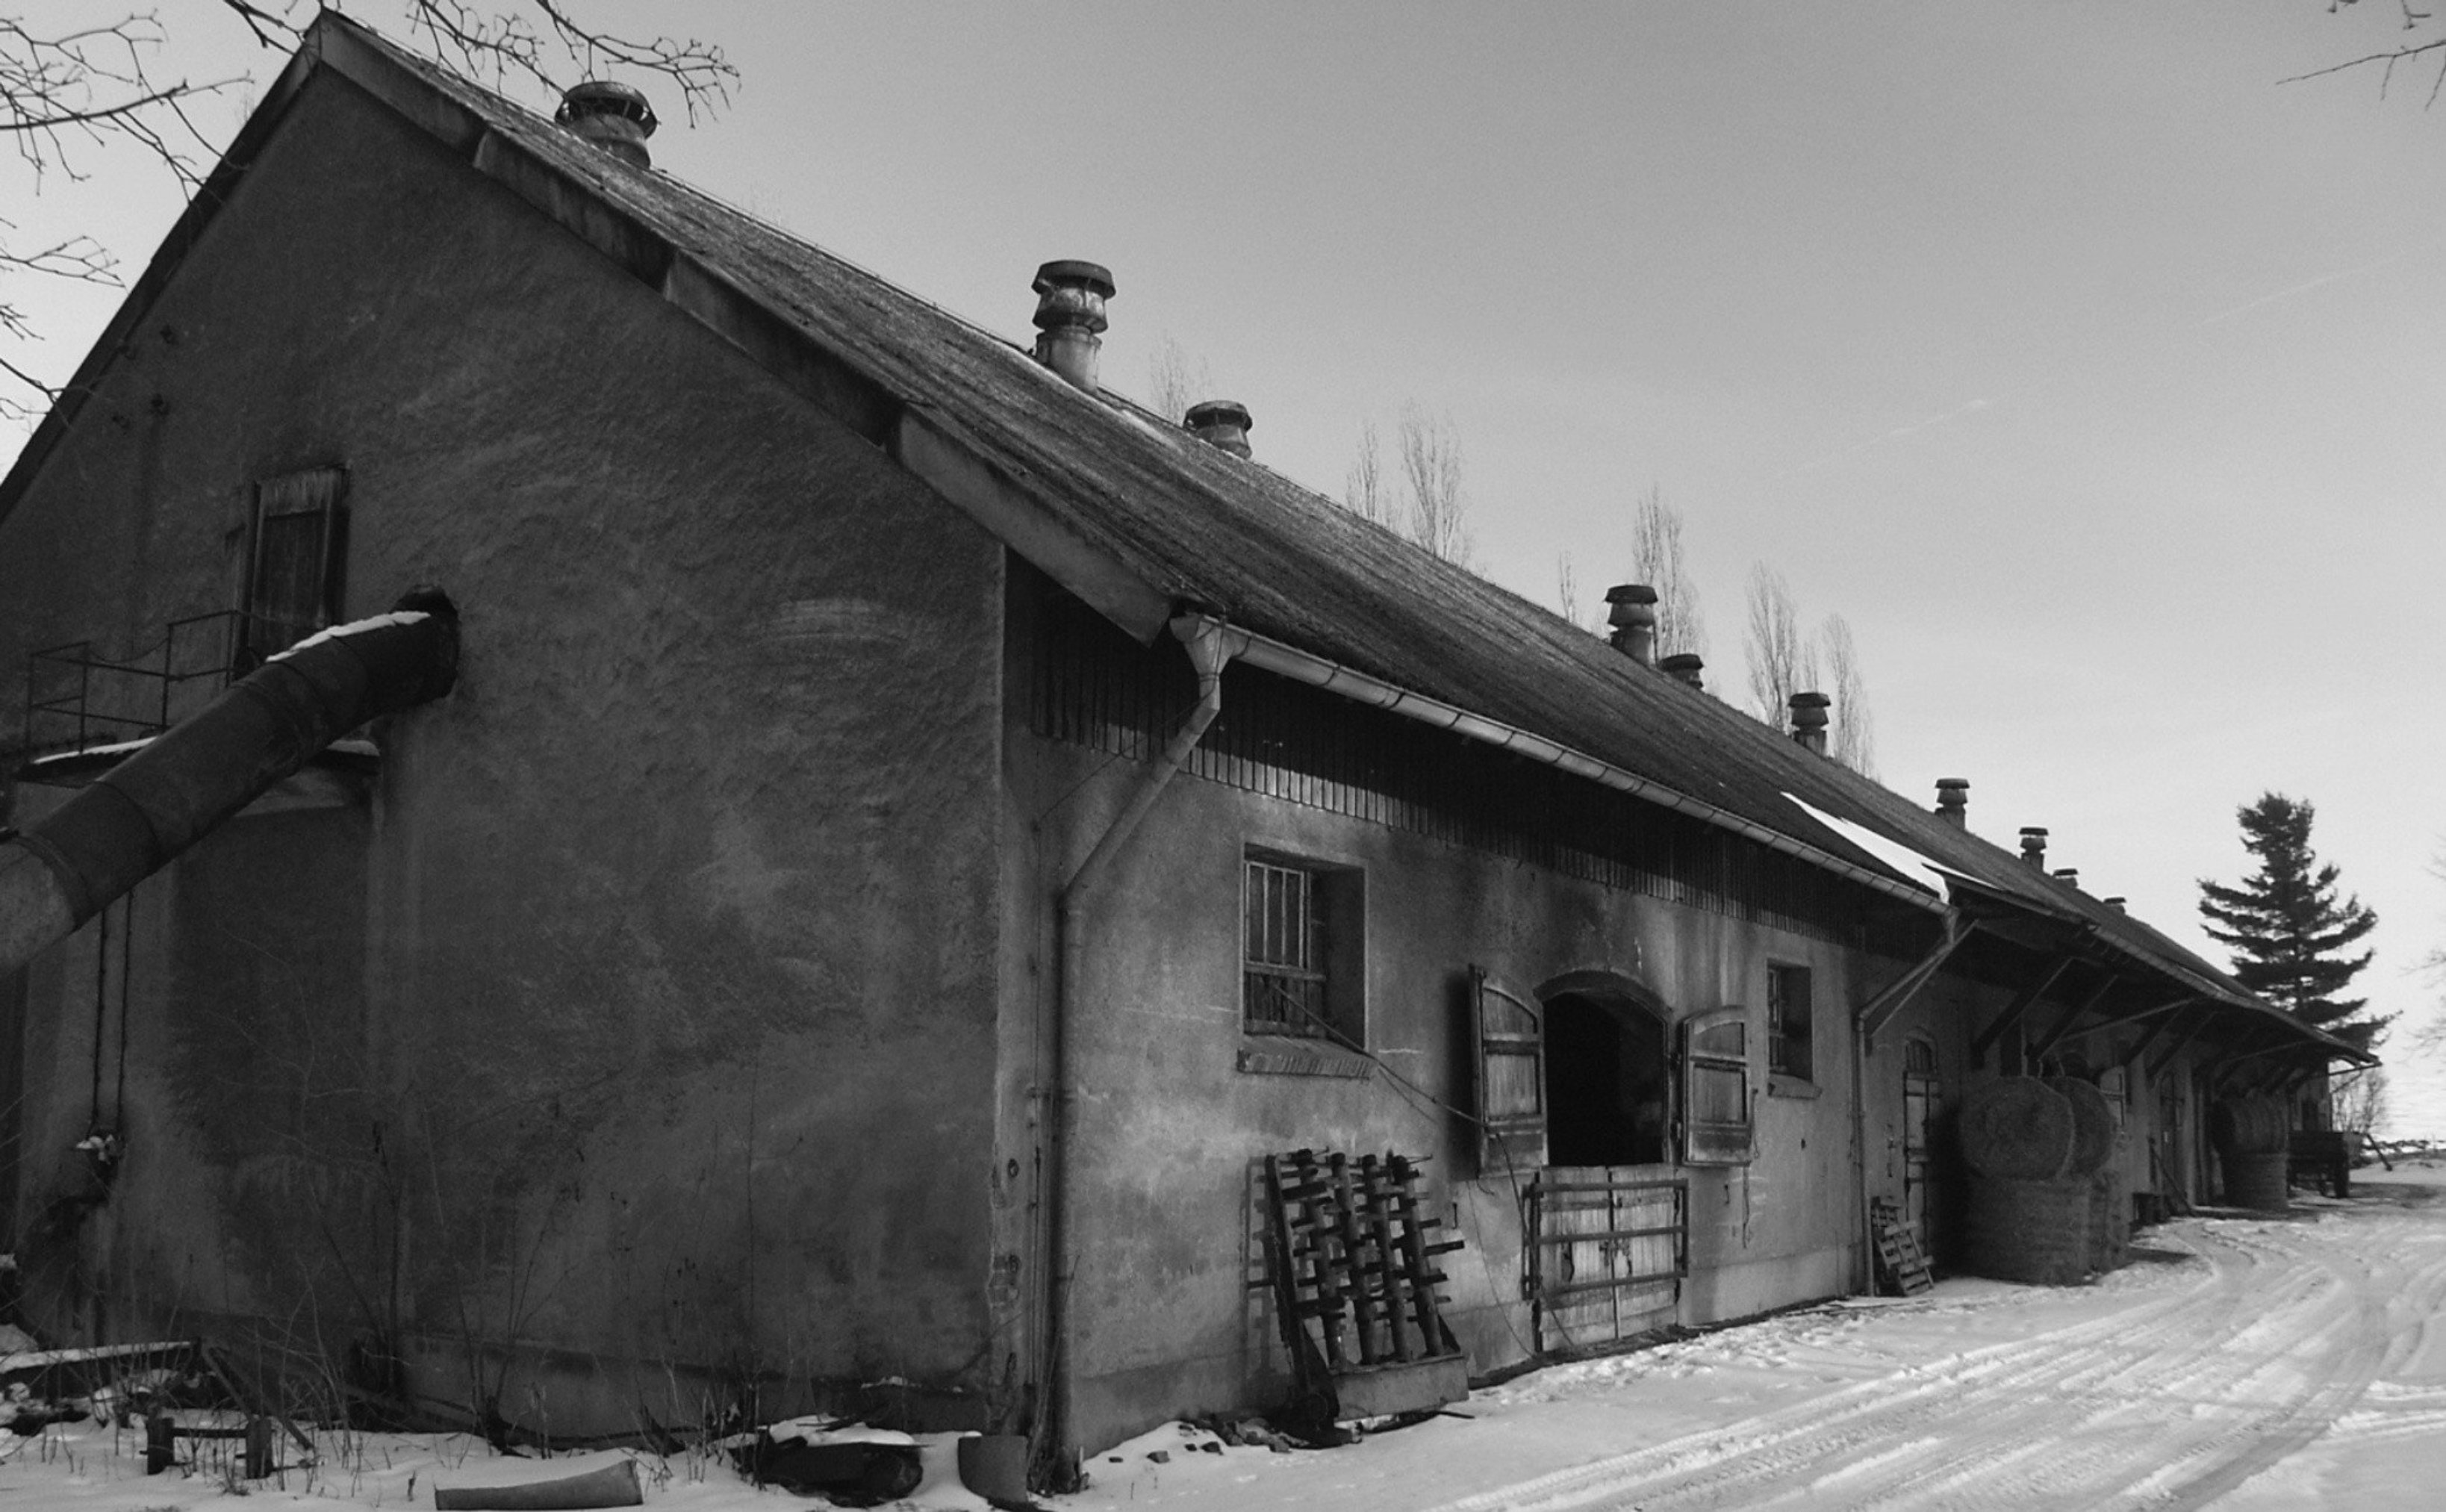
\includegraphics[width=\linewidth]{images/renn03}
    \caption[Der Pferdestall]{Pferdestall in Rennersdorf}
    \label{pferdestallfoto}
\end{figure}


Die Situation der Häftlinge war geprägt durch die gesundheitlichen Folgen des langen Marsches und die Unzulänglichkeiten des provisorischen Lagers. Beides zusammen zehrte an den physischen und mentalen Kräften der Menschen im Lager. Aufgrund der Haftbedingungen kann man, im Vergleich zum Außenlager Görlitz, nicht von einem geregelten, für fast alle geltenden Tagesablauf sprechen. 

Der ehemalige Gefangene Abram Rajchbart\index{p}{Rajchbart, Abram} drückt mit wenigen Sätzen aus, unter welchen Bedingungen die KZ-Gefangenen in Rennersdorf hausten:

\begin{leftbar} 
Hier herrscht Chaos. Wir schlafen auf dem Mist, der mit Stroh bedeckt wird. Die Lebens- und Arbeitsbedingungen sind unmenschlich und entsetzlich. Wir haben keine Möglichkeiten, uns zu waschen und die Wäsche zu wechseln. Das Ungeziefer verbreitet sich, auch die Krankheiten breiten sich aus.\footnote{Aussage von Abram Rajchbart. Jüdisch Historisches Institut Warschau, 301/715.}
\end{leftbar}

Es gab weder ein Krankenrevier noch einen Waschraum. Im Gegensatz zum Görlitzer Lager, existierte keine Wäscherei, Schusterei oder Schneiderei. Die Einrichtung des Lagers reduzierte sich auf eine Küche und eine Latrine aus Birkenholz\footnote{Laut einem Interview  mit Ilse Gießler, Dresden 2005.}. Der Pferdestall diente als \glqq Menschenstall\grqq, ohne Betten, bestenfalls mit etwas Stroh ausgelegt\footnote{Aussage von Max Wachsmann. LArchB B Rep 058 Bd. 6.}. Janusch Oborowicz führt dazu weiter aus:

\begin{leftbar} 
Infolge der in dem Pferdestall bestehenden ungünstigen hygienischen Verhältnisse, hervorgerufen durch die schlechte Luft und die Ausdünstungen des Mistes, haben sich auch die Läuse bei den Häftlingen auffallend vermehrt.\footnote{Aussage von Janusch Oborowicz. BStU MfS ASt 13/48 Bd. 2 / 392.}
\end{leftbar}




\subsection{Die Versorgungslage der Häftlinge}


Janusch Oborowicz\index{p}{Oborowicz, Janusch}:
\begin{leftbar} 
An Verpflegung erhielten wir seinerzeit für acht Häftlinge jeweils 1 Brot und 3/4 Liter halb rohe Gemüsesuppe. Neben den Erschießungen waren infolge der schlechten Ernährung auch weitere Sterbefälle zu verzeichnen.\footnote{Aussage von Janusch Oborowicz, BStU MfS ASt 13/48 Bd. 2 / 392.}
\end{leftbar}

Die Unterernährung war den Gefangenen anzusehen und äußerte sich in der verzweifelten Suche nach Nahrung. Einige der Notleidenden brachten es fertig, so Ilse Gießler\index{p}{Gießler, Ilse}, eine Scheibe Brot von der Straße aufzuheben ohne sich dabei auffällig bücken zu müssen\footnote{Interview mit Ilse Gießler, Dresden, März 2004.}. 

Die ehemalige Rennersdorferin Ilse Gießler\index{p}{Gießler, Ilse} erinnert sich:
\begin{leftbar} 
Fast täglich kamen Häftlinge an unserem Haus vorbei, um beim Bäcker Alter mit einem hierfür gebauten Spezialfahrzeug Brot als Verpflegung für die Häftlinge abzuholen. Eines Tages {[}...{]} war ich Augenzeuge, wie einer der Häftlinge während der Rückfahrt vom Bäcker zum Gute, unmittelbar vor unserem Hause, von einem Posten der SS-Mannschaft mit einem armstarken Knüppel schwer misshandelt wurde, indem er auf ihn einschlug, wobei ihn der noch anwesende Kapo zu halten hatte. Da uns einerseits verboten war, den Häftlingen irgendwelche Nahrungsmittel zu verabreichen oder gar mit ihnen zu sprechen, wir andererseits tiefstes Mitleid mit ihnen empfanden, hat mein Vater eines Tages Äpfel so in den Straßengraben geworfen, dass die Häftlinge sie auf ihrem Rückweg vom Bäcker sehen mussten, wodurch ihnen diese Zuwendung auch tatsächlich gewährt werden konnte. Das Fuhrwerk wurde tatsächlich von ca. 10\textendash{}12 Juden gezogen bzw. geschoben. Alle Häftlinge machten einen verwahrlosten und verhungerten Eindruck
\footnote{Ilse Gießler, am 24.12.1920 in Niederrennersdorf geboren. Die damals 26jährige bewohnte mit ihren Eltern ein heute nicht mehr stehendes Haus an der Hauptstraße (zwischen dem Abzweig Herrnhut und dem Wehr). Ihr Vater war vor 1933 KPD Mitglied, sie selbst ist weder dem Bund Deutscher Mädel, noch einer anderen NS-Organisation beigetreten und wurde deshalb vom damaligen Ortsgruppenleiter für \glqq vogelfrei\grqq~erklärt. Im Jahre 1948 wurde sie als Zeugin im Malitz-Meinshausen-Prozess vorgeladen, jedoch aufgrund der ausreichenden Beweislast gegen die Angeklagten nicht mehr angehört. BStU MfS ASt 13/48 Bd. 2 / 462. Interview mit Ilse Gießler, Dresden, März 2004.} 
\end{leftbar}


Während seit Ankunft der Gefangenen ihre Unterernährung für die Dorfbevölkerung nicht übersehbar war, machte die SS keinen Hehl daraus, im Überfluss zu leben. In jener Zeit hatten selbst die Leute im Dorf nicht übermäßig viel zu essen und empörten sich daher nicht ohne Grund über die Verfütterung von großen Wurstringen an die Hunde der SS\footnote{Laut Aussage mehrerer Zeitzeugen, darunter Ilse Gießler, Helmut Sperling sowie Siegfried und Wolfgang Bittrich.}. Die überschwänglichen SS-Gelage in der Schmidt-Mühle wurden mit Entsetzen durch die Bevölkerung aufgenommen.

Schlomo Graber\index{p}{Graber, Schlomo} erinnert sich der Situation in seinen Memoiren:
\begin{leftbar} 
Die Deutschen schlachteten sich Schafe, warnten uns jedoch, wer sich an den Schafen vergreife, sei des Todes. Hier teilte man uns auch je eine Scheibe Brot zu, die jeder in seinem Brotbeutel wie einen Schatz hütete, um sie krümelweise zu essen. Als ich eines morgens aufwachte -- ich lag zwischen Vater und einem anderen Juden -- spürte ich, dass dieser sich nicht mehr regte, und suchte als erstes sein Brot. Als ich es gefunden hatte, freute ich mich an dem Fund.

An jenem Morgen erschien der älteste Soldat, der die Küche der Deutschen unter sich hatte, und rief mich: \glqq Farzer komm schnell\grqq. Er forderte mich auf, den geschlachteten Schafen das Fell abzuziehen. Von ihm erfuhr ich, dass kranke Schafe für die Häftlinge gekocht werden sollten. Ich fand eine Methode die Schafe krank zu machen. Ich ging in den Pferch, trat einem Schaf in den Bauch, dass es umkippte, und erklärte: \glqq Dies ist krank\grqq. Auf diese Weise bekamen wir nach langem Hungern etwas in den Magen.\footnote{Schlomo Graber: Schlajme, S. 87.}
\end{leftbar}
Die Landarbeiterin Auguste Hergarten\index{p}{Herrgarten, Auguste}: 
\begin{leftbar} 
Die Häftlinge bekamen ein Essen, dass man nicht einmal als brauchbares Schweinefutter bezeichnen kann. Es war furchtbar mit anzusehen, wie die hilflosen armen Menschen immer wieder schwersten Mißhandlungen ausgesetzt waren. Sobald sich eine Gelegenheit bot, steckten wir ihnen zusätzlich etwas Essen zu, obgleich wir selbst nicht viel hatten.\footnote{Auguste Hergarten, am 22.06.1893 in Berthelsdorf geboren. BStU MfS ASt 13/48 Bd. 2 / 464.}
\end{leftbar}


%% Arbeit und Ernährung
Der Rennersdorfer Helmut Sperling erinnert sich, wie sein Vater bei der Lagerleitung um Hilfe beim Fällen einer Eiche bat. Seine Mutter erwartete die Helfer mit einem Teller Schnitten, welcher jedoch von den Bewachern auf dem Erdboden zertrampelt wurde.


%%%%%%%%%%%%%%%%%%%%%%%%%%%%%%%%%%%%%%%%%%%%%%
\subsection{Zwangsarbeit auf dem Gut Oberrennersdorf}
Der Bericht des Zeitzeugen Helmut Sperrling legt die Vermutung nahe, die Häftlinge seien auch in Rennersdorf von der Zwangsarbeit verschont geblieben. Dies wird jedoch in nur in sehr wenigen Überlieferungen ehemaliger Gefangener bezeugt. Ein Großteil der Menschen war nach dem anstrengenden Marsch nach Rennersdorf physisch und psychisch kaum noch in der Lage zu arbeiten. Angesichts dessen wird nur eine Minderheit, vor allem aber Frauen, zur Arbeit herangezogen worden sein\footnote{Vor und nach der Evakuierung gibt es übereinstimmende Zeugenaussagen, wonach die Frauen in einer eindeutig besseren körperlichen Verfassung waren als die Männer.}.
Die Art der Arbeit richtete sich nach den örtlichen Erfordernissen der im Hof betriebenen Landwirtschaft.
Damals arbeitete neben vielen anderen auch Liesbeth Sägners\index{p}{Sägner, Liesbeth} Mutter im Gut Oberrennersdorf als Landarbeiterin. Sie wusste zu berichten, dass die Häftlinge mit ihr und anderen Rüben sortieren mussten. Obwohl sie sich in einem erbärmlichen Zustand befanden, war es ihnen verboten von den Möhren zu essen, weshalb Frau Sägners Mutter ihnen aus Mitleid mehrmals einen Kanten Brot bei der Arbeit zuschob\footnote{Laut Liesbeth Sägner.}. 
Abram Rajchbart\index{p}{Rajchbart, Abram} beschreibt die Arbeitsbedingungen insgesamt als unmenschlich und entsetzlich\footnote{Aussage von Abram Rajchbart. ZIH 301/715.}. Die Annahme der Historiker Gräfe / Töpfer und Zg\l obicki, wonach in Rennersdorf Schanzarbeiten verrichtet wurden, konnte in den zahlreichen Überlebendenberichten nur gegenteilige Bestätigung finden, zumal es in ganz Rennersdorf keine Überreste solcherlei Arbeit gibt. Aller Wahrscheinlichkeit nach handelte es sich hierbei um eine Verwechslung mit den bei der Rückkehr nach Görlitz befohlenen Schanzarbeiten.\footnote{Vgl. Gräfe / Töpfer: Die Konzentrationslager auf dem Territorium des heutigen Sachsens. Vgl. auch: Roman Zg\l obicki: Obozy i cmentarze Wojenne w Zgorzelcu.}. 




%%%%%%%%%%%%%%%%%%%%%%%%%%%%%%%%%%%%%%%%%%%%%%
\subsection{Kontakt zur Dorfbevölkerung}
Rennersdorf hatte während des Krieges nur wenige hundert Einwohner, die fast alle miteinander bekannt waren. Die Neuigkeit von der Ankunft der erbärmlich ausschauenden Häftlinge am 23. Februar 1945 verbreitete sich also rasch, zumal die Kolonne zuvor auf gut zwei Kilometern die Hauptstraße des Ortes passierte. 

\glqq Jeder wusste es\grqq\footnote{Laut Ilse Gießler und vielen anderen teils ehemaligen Rennersdorfern.}. Die Neuigkeit von der Ankunft der erbärmlich ausschauenden Häftlinge verbreitete sich rasch. Den Pferdestall, in dem die Häftlinge untergebracht waren, konnte man sehr gut von der am Eichler vorbeiführenden Straße zwischen Herrnhut\index{o}{Herrnhut} und Bernstadt\index{o}{Bernstadt} / Großhennersdorf\index{o}{Großhennersdorf} einsehen. Ilse Gießler berichtete, wie sie während eines Waldspazierganges auf dem Berg Eichler die abgemagerten Gefangenen beobachten konnte. Insbesondere jene Rennersdorfer, die auf dem Gutshof wohnten oder arbeiteten, konnten sich der Präsenz der Gefangenen keinesfalls verschließen. Offensichtlich hielt die SS Appelle im Hof des Gutes ab, bei denen es immer wieder zu Folterungen kam\footnote{Interview mit den Brüdern Bittrich, die einst als kleine Jungen im Alter von 4 und 8 Jahren Zeuge der Gewalt wurden. Rennersdorf, 29.03.2004.}. Die SS - seit dem Todesmarsch durch eine ukrainische Einheit verstärkt - provozierte durch ihren Umgang mit den Gefangenen bei den Hofbewohnern eine Angst, selbst in Mitleidenschaft gezogen zu werden. Die Rennersdorfer sollten sehen, was ihnen blühte, wenn sie den Gefangenen Mitleid entgegen brachten.

%\begin{landscape}
\mymapfigure[karterennersdorf]{map_rennersdorf}{}{Rennersdorf}{Rennersdorf}{0}{33}%0.515
%\end{landscape}

Bereits bei der Ankunft, als die Gefangenen das Hoftor passierten, deutete sich alles an. Es kam zu einer ersten Erschießung vor den Augen einiger Frauen und Kinder. Janek Schilid  sagte 1948 dazu:

\begin{leftbar} 
Da vor dem Erreichen des Dorfes ein ziemlich steiler Berg zu überwinden war, da einer der Häftlinge zu schwach war, den sich hieraus ergebenen körperlichen Anforderungen gerecht zu werden und zusammen sank, wurde er an der Straße durch angehörige des Wachpersonals erschossen. \footnote{Janek Schilid. BStU MfS ASt 13/48 Bd. 2 / 397.}
\end{leftbar} 

%Weitere Erschießungen beobachten Kinder hinter dem Hof an einem Wiesenweg\footnote{Laut Helmut Sperling.}. Von weitem sichtbar hatte die SS an einer Linde neben dem Pferdestall einen Häftling aufgehangen\footnote{Laut Wolfgang und Siegfried Bittrich.}. 

\newpage
Die Unterernährung war den Gefangenen anzusehen und äußerte sich in der verzweifelten Suche nach Nahrung. Dabei ersuchten sie auch Rennersdorfer um Hilfe. Jedoch stets unter Gefahr, von der SS erwischt zu werden, wie jene beim Bauer Schönfelder\index{p}{Schönfelder}\footnote{Vgl. Katja Junge: Der Todesmarsch vom KZ-Außenlager Biesnitzer Grund nach Rennersdorf 1945, unveröffentlichtes Manuskript, S. 6.}.

Außerhalb des Gutshofes und bei der Abholung des Brotes beim Bäcker\index{p}{Alter} kamen die Häftlinge jedoch kaum in Kontakt mit der Dorfbevölkerung. 

%% Löwe
Bemerkenswert ist die Begegnungen im Hause der Familie Löwe, welche unweit vom SS-Quartier in der Schmidt-Mühle wohnte: Joachim Löwes Mutter war an Fieber erkrankt und man befürchtete, eine Epidemie könntex sich ausbreiten. Der Arzt im Nachbarort Herrnhut war verhindert, weshalb sich der NSDAP-Ortsgruppenleiter nach einem Arzt unter den jüdischen Häftlingen erkundigte und fündig wurde. Die Behandlung durch einen jüdischen Arzt galt in jener Zeit als \quotedblbase{}Rassenschande\textquotedblleft{}. Seit dem Erlass der Nürnberger Gesetze (15.09.1933) war es jüdischen Ärzten untersagt, \quotedblbase{}Arier\textquotedblleft{} zu behandeln. Trotzdem gestattete die Lagerleitung dem Arzt Frau Löwe zu behandeln. Mit einer Medikamententasche erschien er im Haus der Löwes. Einer der beiden ihn begleitenden Bewacher wollte zunächst der Behandlung beiwohnen, erst als Frau Löwe mit einem Fingerzeig auf das Bild ihres im Krieg gefallenen Gatten hindeutete, verließ der SS-Mann die Stube. Der Arzt war mit Medikamenten sowie notwendigen Utensilien ausgestattet und somit in der Lage der Erkrankten bei diesem und zwei weiteren Hausbesuchen zu helfen. Die Löwes arrangierten sich, indem sie ihm ein paar Stullen Brot gaben, die er nach anfänglichem Zögern in seiner Hose versteckte.\footnote{Interview mit Joachim Löwe, Rennersdorf 2004 und 2005. }




%%%%%%%%%%%%%%%%%%%%%%%%%%%%%%%%%%%%%%%%%%%%%%

\subsection{Die SS in Rennersdorf}
Die Kommandostruktur der SS war in Rennersdorf dieselbe wie zuvor in Görlitz. Erich Rechenberg\index{p}{Rechenberg, Erich} als Lagerkommandant verblieb in Görlitz und kam nur gelegentlich nach Rennersdorf. Lagerführer Zunker\index{p}{Zunker, Winfried}, Rapportführer sowie die älteren SS-Leute und die als grausam beschriebenen ukrainischen SS-Männer bezogen in Rennersdorf Quartier. Ein Großteil der Wachmannschaften wohnte auf dem Gut, ein Teil soll auch bei Wunderlichs und andere bei Wenzels auf dem Gittelberg logiert haben\footnote{Interview mit Christa Schubert, Berthelsdorf, den 01.04.2005. Die Familien Wunderlich und Wenzel konnten nicht mehr eindeutig ausfindig gemacht werden.}. Zumindest der Lagerführer\index{p}{Zunker, Winfried} bezog während dieser Zeit mit seinen Hunden und seinen bediensteten Häftlingen (\glqq Stiefelputzer\grqq) die Schmidt-Mühle am Fuchsberg\footnote{Interview mit Helmut Sperling, der in unmittelbare Nähe wohnte. Rennersdorf 23.12.2003.} (Bild ~\mypicsref{schmidtfoto}). 


\begin{figure}[htb]
    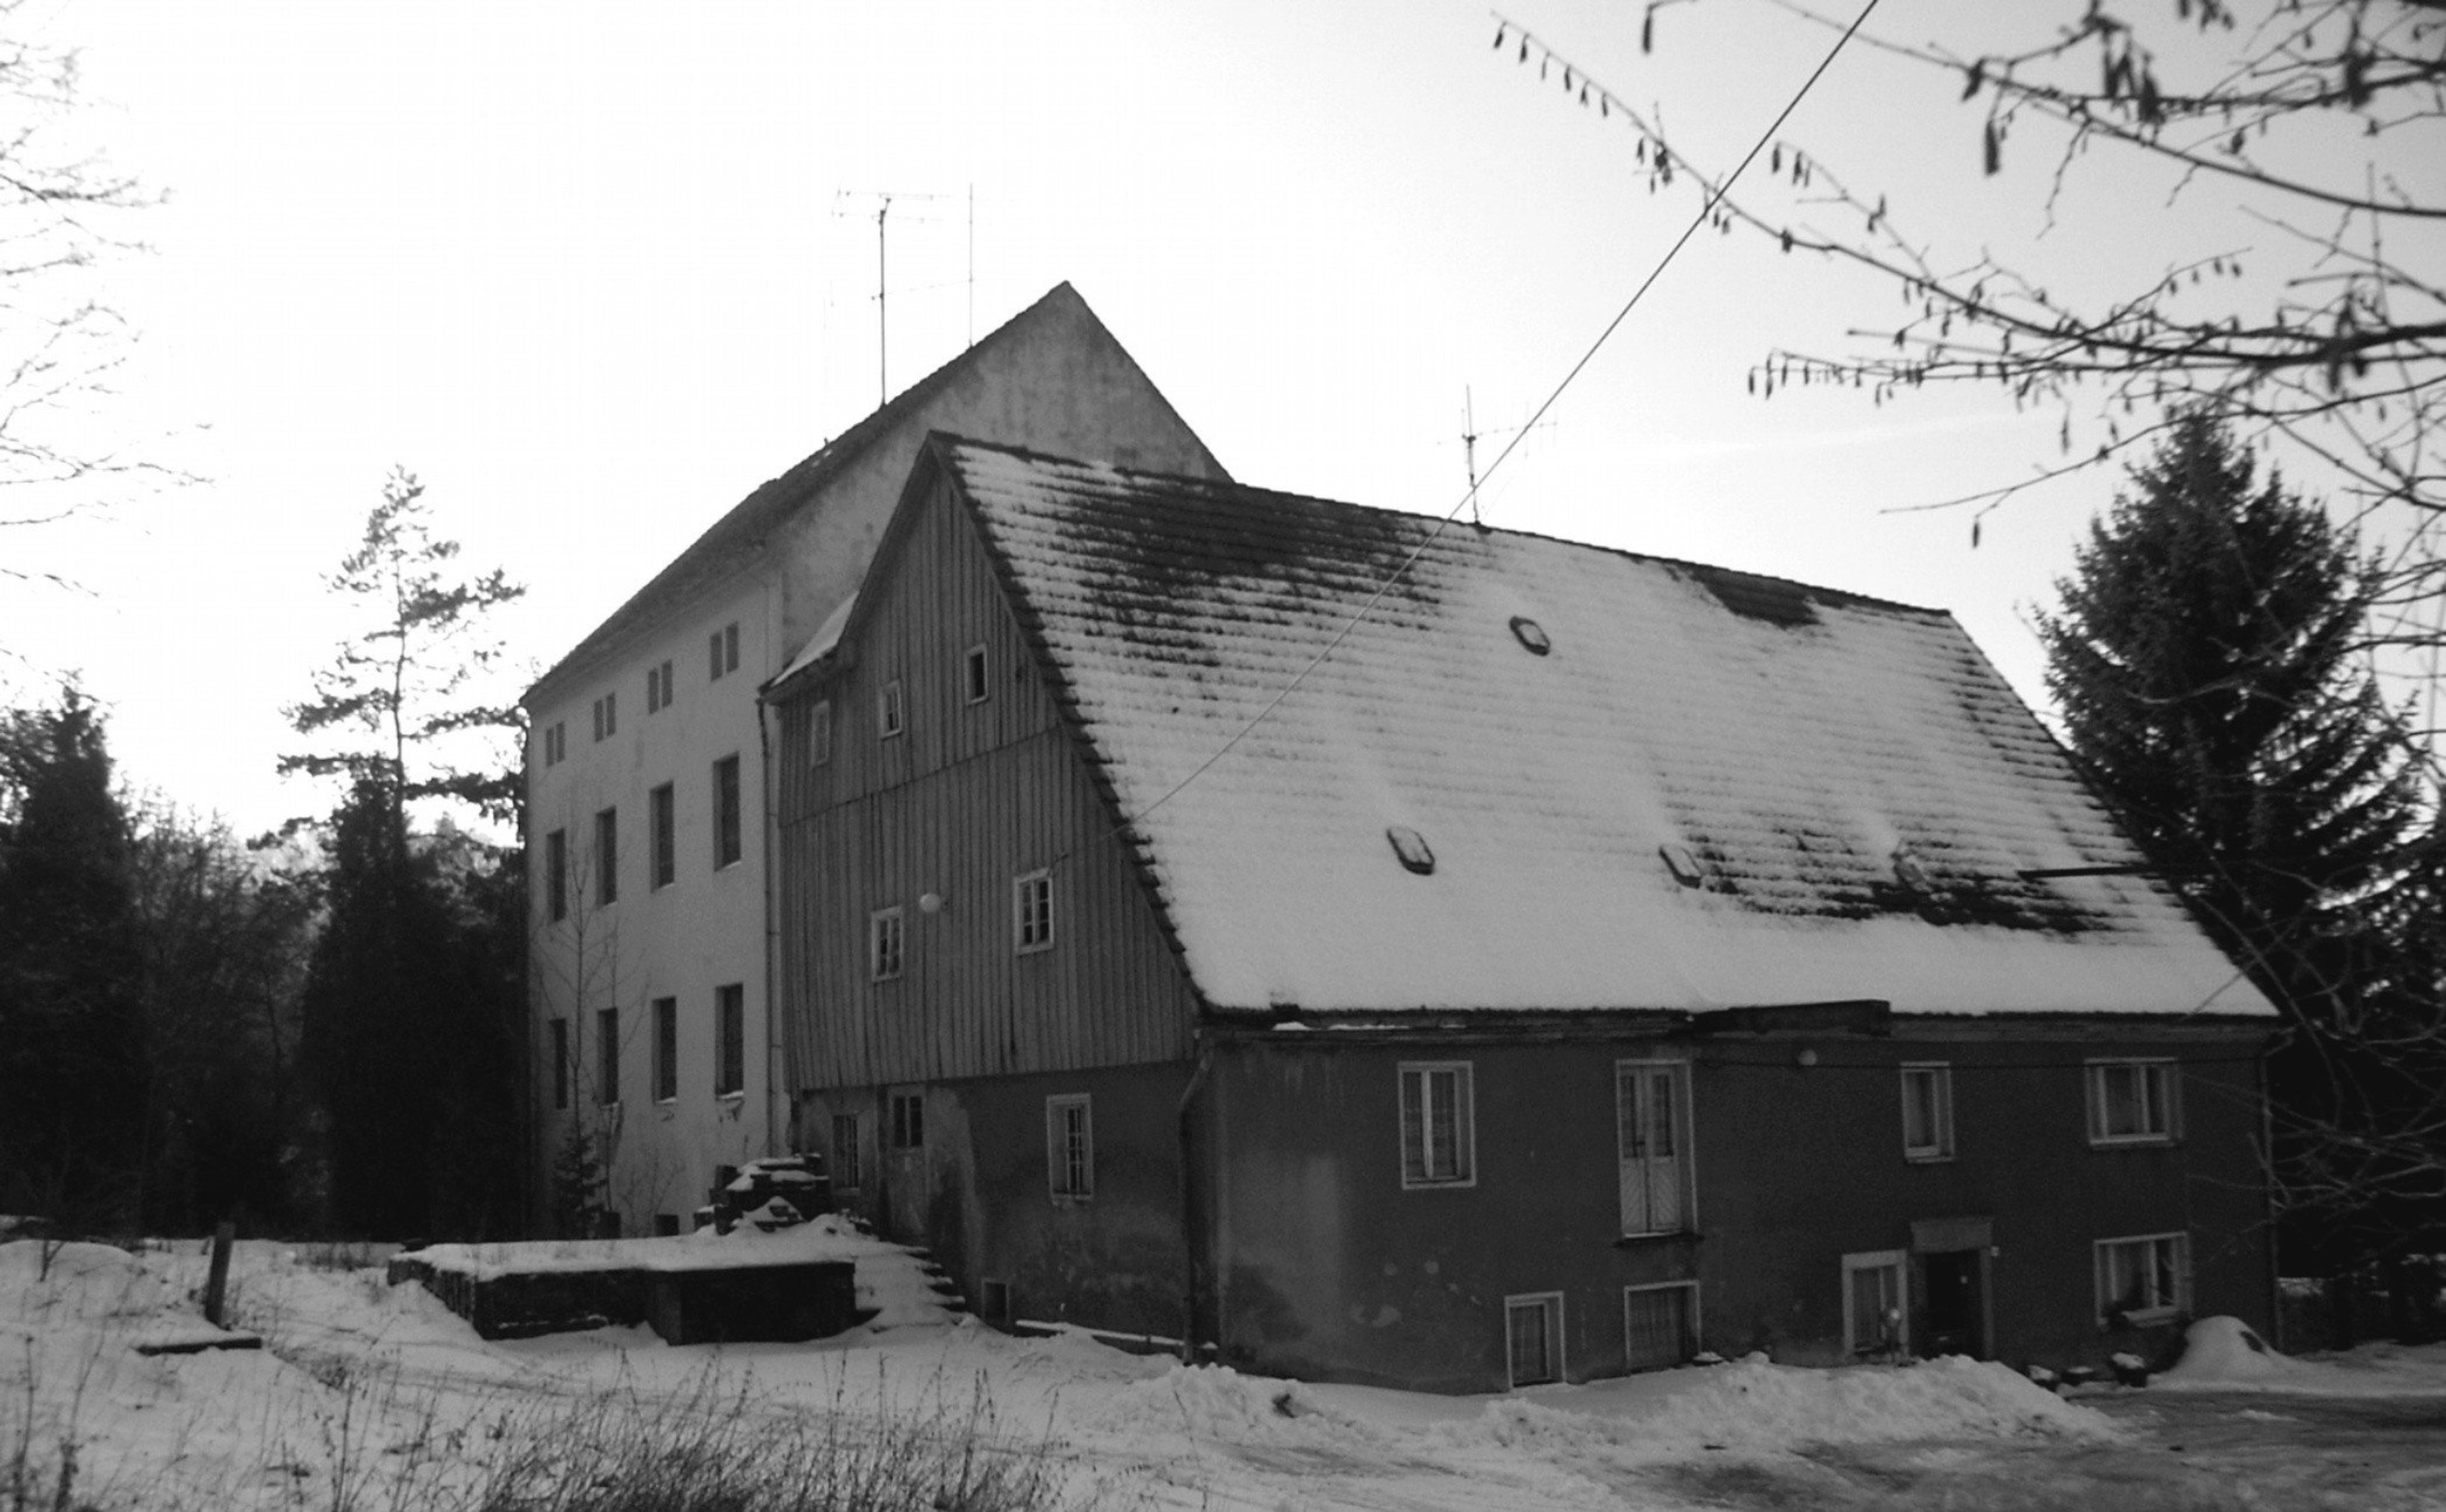
\includegraphics[width=\linewidth]{images/renn02}
    \caption{Schmidt-Mühle}
    \label{schmidtfoto}
\end{figure}



%%%%%%%%%%%%%%%%%%%%%%%%%%%%%%%%%%%%%%%%%%%%%%
\subsection{SS-Terror in Rennersdorf}

Wie bereits erwähnt, begann das Morden schon bei Ankunft der Gefangenen im Gutshof. Eine weitere Erschießung erfolgte in der darauf folgenden Nacht, als ein Häftling die Unterkunft zum Austreten verließ\footnote{Janek Schilid. BStU MfS ASt 13/48 Bd. 2 / 397.}. 

Isaac Weintraub\index{p}{Weintraub, Isaac}:
\begin{leftbar} 
Es gab keine Krankenbaracke. So wurde angeordnet, dass diese Häftlinge von der begleitenden Wachmannschaft, die teilweise aus ukrainischer SS bestand, erschossen wurden. Die Häftlinge wurden mit Karabinern, die aus einer Entfernung von 50\,m auf sie gerichtet wurden, erschossen und in der Feldtoilette begraben.\footnote{Aussage von Isaac Weintraub. LArchB B Rep 058 Bd. 3/4}
\end{leftbar}
Auguste Hergarten\index{p}{Herrgarten, Auguste}: 
\begin{leftbar} 
Ich war als Landarbeiterin auf dem Gut Oberrennersdorf beschäftigt und wiederholt Zeuge, wie die Kapos die Häftlinge wegen den kleinsten Geringfügigkeiten Schläge verpassten. Mir wurde auch von Häftlingen erzählt, dass wiederholt Juden durch das SS-Wachpersonal erschossen worden sind. Sie wurden hinter dem Remontestall vergraben [...]
Unter ihnen befand sich auch ein 18-jähriger Häftling, der erschossen wurde, weil er sich aus der Rübenmiete eine Runkelrübe beschafft hat, um sie zu essen.\footnote{Auguste Hergarten BStU MfS ASt 13/48 Bd. 2 / 464.}
\end{leftbar}


\begin{figure}[htb]
    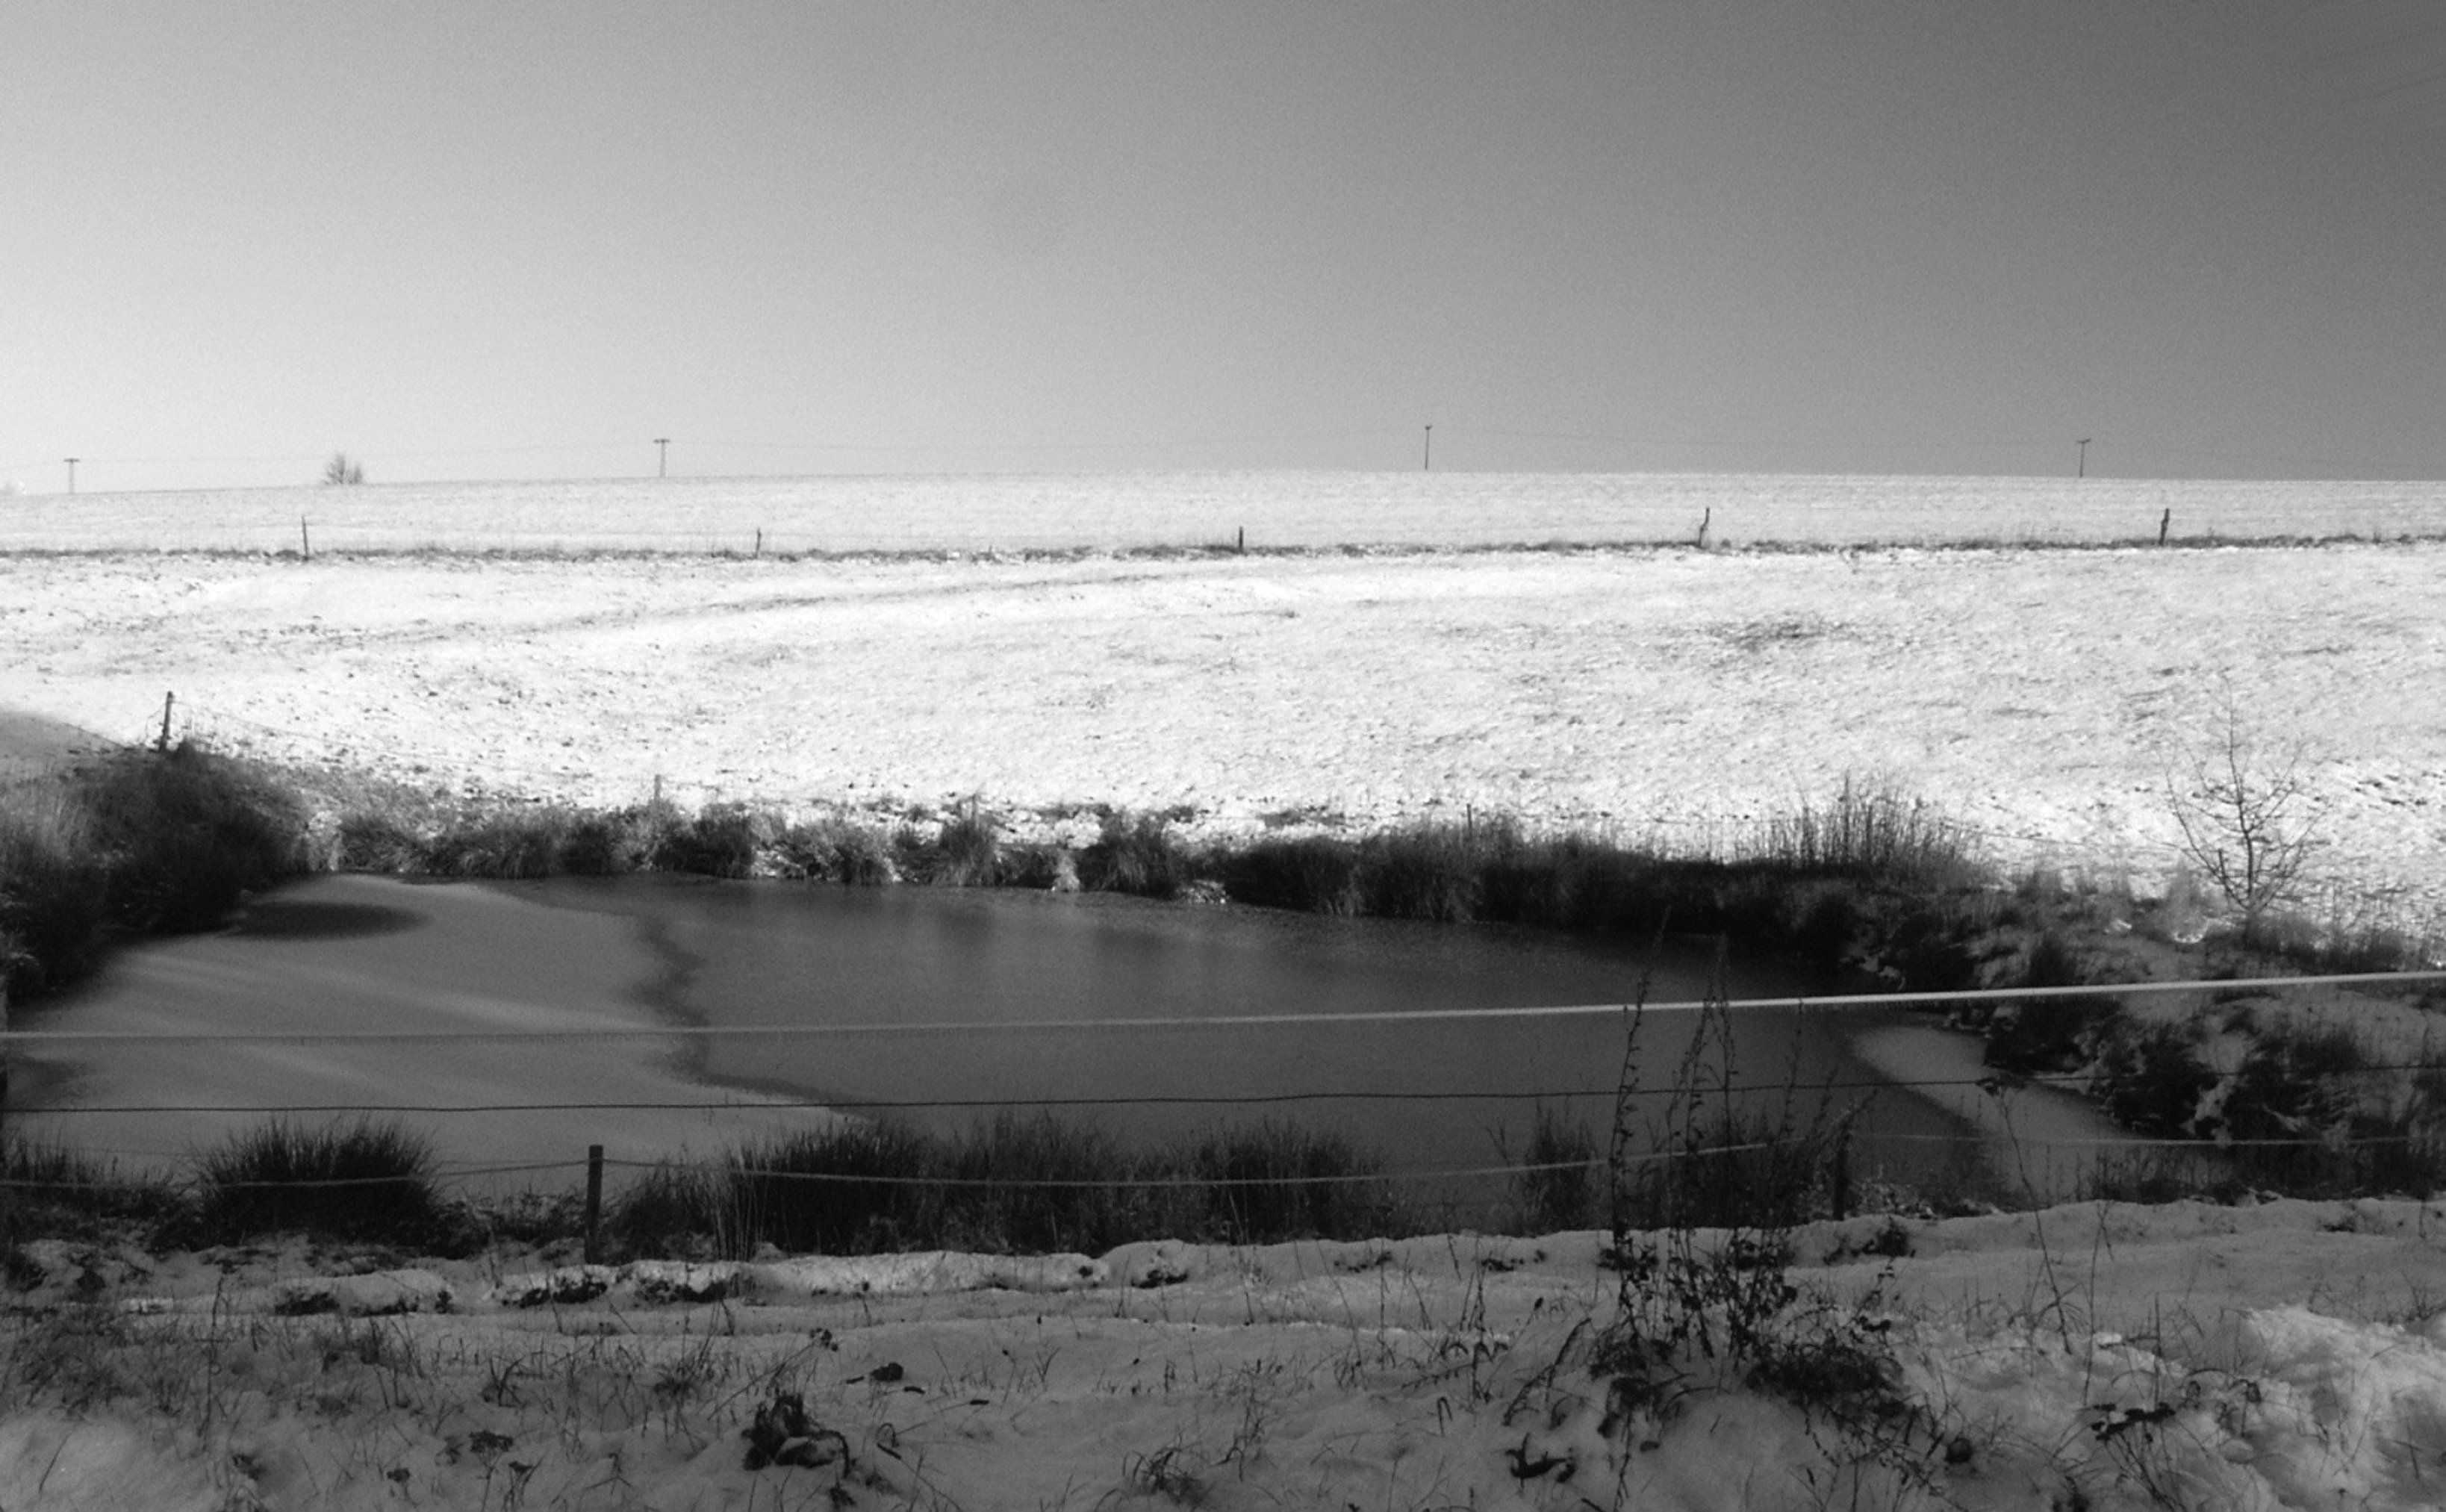
\includegraphics[width=\linewidth]{images/renn04}
    \caption[Wiesenweg / Teich]{Der einstige Erschießungsort am Wiesenweg ist heute ein Teich.}
    \label{wiesenweg}
\end{figure}


Helmut Sperling\index{p}{Sperling, Helmut} verbrachte in Kindheitstagen viel Zeit bei einem Freund auf dem Gutshof und erinnert sich an mehr als vier Exekutionen am Damm eines Wiesenweges (Bild ~\mypicsref{wiesenweg}), an dessen Stelle sich heute ein Löschteich befindet. Nachdem die zum Tode Bestimmten ihr eigenes Grab notdürftig ausgehoben hatten, wurden sie an den Rand der Grube gegenüber dem Pferdestall an einem Wiesenweg gesetzt und durch einen Genickschuss getötet\footnote{Helmut Sperling. Interview vom Dezember 2003 in Rennersdorf.}. Dem Gutsverwalter Lehmann\index{p}{Lehmann, Reinhold} sagt man nach, dass er den Abraum, der beim Fegen des Hofes zusammen kam, auf die Gräber am Wiesenweg kippen ließ, um somit die Vorkommnisse auf seinem Hof zu vertuschen. Die sowjetische Militärkommandantur verhaftete ihn deshalb nach Kriegsende. 


%%%%%%%%%%%%%%%%%%%%%%%%%%%%%%%%%%%%%%%%%%%%%%
Wenn auch als einziger, erinnert sich Samuel Kessler\index{p}{Kessler, Samuel} an eine Erschießung eines Zivilarbeiters:
\begin{leftbar} 
Während des Evakuierungsmarsches war ich Augenzeuge der Erschießung eines entflohenen polnischen Kriegsgefangenen, der von der örtlichen Polizei in Rennersdorf dem KL [Konzentrationslager] überstellt wurde. [\dots]

Es erschien dann Gendarmarie, die einen aus einem Kriegsgefangenenlager geflüchteten Mann, vermutlich ein Pole, dem [Lagerführer] Zunker\index{p}{Zunker, Winfried} vorführte. Es war der Zeitpunkt, als wir auf dem Zufahrtsweg zu dem Gestüt in die Ställe eingeschleust werden sollten. Ich bemerkte, dass Zunker wieder sehr aufgeregt war. Ich saß auf dem Bock des Pferdefuhrwerks und befand mich in unmittelbarer Nähe des Geschehens. Zunker\index{p}{Zunker, Winfried} wusste offensichtlich nichts mit dem herangeführten Häftling anzufangen und wollte ihn auch nicht haben. Er stellte ihn dann einige Meter entfernt von sich ab, drehte sich um, zog plötzlich die Pistole und schoß mit 3--4 Schüssen dem Häftling in den Körper. Dieser fiel sofort um und war tot. Auf dem danebenliegenden Feld ist dann dieser Gefangene von Mithäftlingen verscharrt worden. Der Gefangene war damals so um die 30--40 Jahre alt und trug Zivilkleidung.\footnote{Aussage von Samuel Kessler\index{p}{Kessler, Samuel}, LArchB B Rep 058 Bd. 1 und 6.}
\end{leftbar}
 








%%%%%%%%%%%%%%%%%%%%%%%%%%%%%%%%%%%%%%%%%%%%%%
\section{Die Rückkehr nach Görlitz}
Nach den Rückschlägen bei den Kämpfen um Lauban\index{o}{Lauban} verlagerten sich die militärischen Operationen der Roten Armee ab dem 8. März in Richtung Berlin\index{o}{Berlin}. Folglich stabilisierte sich die Frontlage bei Görlitz. \glqq Die Rüstungsbetriebe holten ihre Arbeitslager, die sie evakuiert hatten, zum größten Teil wieder zurück. Dasselbe trifft auch für das Arbeitslager Biesnitzer Grund zu.\grqq, heißt es in einer Aussage des Görlitzer Kreisleiters Malitz\index{p}{Malitz, Dr. Bruno}\footnote{BStU MfS ASt 13/48 Bd. 2 / 172.}. 
Malitz\index{p}{Malitz, Dr. Bruno} versuchte die Verantwortung für die gesamte Evakuierung auf die WUMAG abzuwälzen, obwohl die von ihm mit getragenen Ambitionen Görlitz zur Festung auszubauen, ausschlaggebend für den Rückmarsch der Häftlinge waren. Auch der Lagerkommandant Rechenberg\index{p}{Rechenberg, Erich} und die nach Reichenau (Rychnov u Jablonce nad Nisou, Tschechien)\index{o}{Reichenau} verlegte Kommandantur des Stammlagers musste informiert gewesen sein. 

Der Abzug der Gefangenen am 8. März 1945 bedeute gleichzeitig die Auflösung des 13 Tage zuvor entstandenen Außenlagers Rennersdorf. 

\begin{leftbar} 
Vor dem Abmarsch gab es einen Appell. Solche Appelle waren etwas Alltägliches. Die Deutschen wollten wissen, wie viele Häftlinge noch übrig waren. [...] Sie fragten, wer marschunfähig sei. Es meldeten sich rund 100 Leute, die per Lastwagen ins Lager Görlitz gefahren wurden. Als wir dort ankamen, fanden wir sie lebend vor.\footnote{Schlomo Graber: Schlajme, S. 87. Siehe auch: Aussage von Dov Bernard Levi\index{p}{Levi, Dov Bernard}, welcher selbst mit dem Lastwagen nach Görlitz zurück kam. LArchB B Rep 058 Bd. 5.}
\end{leftbar}

Der Großteil der Gefangenen ging zu Fuß und verließ Rennersdorf Richtung Niederdorf. Obwohl Schlomo Graber\index{p}{Graber, Schlomo} von gutem Wetter schreibt, welches das \glqq Gehen erleichterte\grqq, herrschten immer noch winterliche Temperaturen. Janusch Oborowicz\index{p}{Oborowicz, Janusch} dazu:
\begin{leftbar} 
Die Straßen waren während unseres Marsches sehr stark vereist und wir konnten nicht verhindern, dass ein Fahrzeug ins Rutschen kam, als wir eine steil abfallende Straße passierten. Bei der Gelegenheit hat sich der Lagerführer dermaßen aufgeregt, dass er mit seiner Pistole anfing zu schießen und zwei unserer Leute verletzte.\footnote{Janusch Oborowicz. BStU MfS ASt 13/48 Bd. 2 / 393.}
\end{leftbar}
Janek Schilid\index{p}{Schilid, Janek} fügt hinzu:
\begin{leftbar} 
Der von uns bisher benützte Knüppel zum Bremsen auf abschüssigen Straßen reichte nicht aus, dass Fuhrwerk zu einer angemessenen, gemäßigten Geschwindigkeit zu halten, so dass es einem Häftling über die Beine und über den Bauch gefahren ist, was seinen Tod zur Folge hatte.\footnote{Janek Schilid. BStU MfS ASt 13/48 Bd. 2 / 397.}
\end{leftbar}
Überlebendenberichten zufolge sollen abgesehen von diesem Unfall während des Rückmarsches keine oder nur vereinzelt Menschen ums Leben gekommen sein\footnote{Unter anderem die Aussage von Maximilian Brandt, LArchB B Rep 058 Bd. 3. Vgl. auch: Schlomo Graber: Schlajme, S. 88.}.



%%%%%%%%%%%%%%%%%%%%%%%%%%%%%%
\begin{fshaded}\vspace{-.5cm}\subsection*{Nutznießer des Todesmarsches}
Als Frauen, Kinder, Alte und Schwache die Stadt Görlitz auf Befehl vom NSDAP Kreisleiter\index{p}{Malitz, Dr. Bruno} verlassen mussten, bot der Lagerführer Winfried Zunker\index{p}{Zunker, Winfried} der Görlitzerin Ursula Taube\index{p}{Taube, Ursula} an, zusammen mit der Häftlingskolonne am 18.02.1945 die von der Roten Armee bedrohte Stadt zu verlassen. Sie war zu dem Zeitpunkt schwanger und hatte keine Fahrtgenehmigung für die Eisenbahn bekommen. Neben Frau Taube konnte ihre Verwandtschaft mütterlicherseits, bestehend aus Mutter, Tante und Großeltern, den Weg antreten. Ebenso eine Flüchtlingsfrau mit ihrem 1$\frac{1}{2}$jährigen Kind.

\begin{leftbar}
In den frühen Nachmittagsstunden begaben wir uns in das Lager Biesnitzer Grund, wo die Häftlinge bereits zum Abmarsch angetreten standen. Hier wurden uns von Zunker\index{p}{Zunker, Winfried} zwei weibliche Häftlinge zum Schieben des Kinderwagens, den wir mit uns führten, zugeteilt und wir setzten uns an die Spitze des Zuges mit den Häftlingen in Richtung Kunnerwitz\index{o}{Kunnerwitz} über Biesnitz in Bewegung. Der Abstand zwischen uns und den Häftlingen schwankte zwischen 300 und 400 Metern.\footnote{Aussage von ursula Taube. BStU MfS ASt 13/4.}
\end{leftbar}
Ihnen war laut eigener Aussage bewusst, dass die Häftlinge aufgrund ihrer Unterernährung nur so langsam voran kamen. Bei der Ankunft in Kunnerwitz\index{o}{Kunnerwitz} nahmen sie Quartier in einem Privathaus, während die Häftlinge in die Scheune des Bauern Fünfstück\index{p}{Fünfstück} eingepfercht wurden. Das Betreten des Hofes war ihnen während der drei Tage und zwei Nächte untersagt. Beim Abrücken erfuhren sie von dem Aufräumungskommando durch Zunker\index{p}{Zunker, Winfried}, dessen Funktion er ihnen im wörtlichen Sinne erklärte. Einer der Wachleute erläuterte der Familie einige Zeit später, was in Wirklichkeit unter \glqq aufräumen\grqq~zu verstehen war, nämlich die Beseitigung von Leichen. Ursula Taube\index{p}{Taube, Ursula} hatte ein offenbar sehr gutes Verhältnis zu Zunker, weshalb sie ihn daraufhin zur Rede stellte. Entsetzt über den Verrat konnte er die Gräuel nicht länger leugnen und gestand die Erschießung kranker, gehunfähiger Häftlinge ein. 
Vom Abend desselben Tages berichtet sie: \glqq Während die Häftlinge in der Scheune des Bauern Göbel\index{p}{Göbel} untergebracht waren, schliefen ich und meine Mutter in der Mansarde des Wohnhauses.\grqq\footnote{Aussage von Ursula Taube. BStU MfS ASt 13/4.} In Rennersdorf ergab sich eine ähnliche Situation, wobei ihnen der Rennersdorfer Bürgermeister eine Aufenthaltsgenehmigung, und die damit verbundene Zuteilung von Lebensmittelkarten versagte. Da alle sieben Personen ebenso lang in Rennersdorf verblieben, wie die Häftlinge, muss davon ausgegangen werden, dass sie sich nur auf Kosten der KZ-Gefangen ernährt haben konnten.\grqq~Zumindest Frau Taube fuhr im PKW mit Zunker und einem nicht namentlich erwähnten Feldwebel nach Görlitz zurück; nicht jedoch ohne die auf dem Fußmarsch befindliche Kolonne zu überholen und deren erbärmliche Verfassung zu registrieren: 
\begin{leftbar} 
Die Fuhrwerke wurden hierbei von den Frauen gezogen, während die Männer teilweise derartig erschöpft waren, dass sie auf diesen von den Frauen gezogenen Fuhrwerken saßen und lagen.\footnote{Aussage von Ursula Taube. BStU MfS ASt 13/4.}
\end{leftbar}
In den darauf folgenden Tagen und Wochen bis kurz vor Kriegsende stand Frau Taube in engem Kontakt mit dem Lagerführer Zunker\footnote{Aussage von Ursula Taube. BStU MfS ASt 13/4.}.

%Im Übrigen sei es dem Leser überlassen, das Verhalten von Frau Taube kritisch zu diskutieren.
\end{fshaded}

\newpage

